\documentclass[
	% -- opções da classe memoir --
	12pt,				% tamanho da fonte
	oneside,			% para impressão em verso e anverso. Oposto a oneside
	a4paper,			% tamanho do papel. 
	% -- opções da classe abntex2 --
	%chapter=TITLE,		% títulos de capítulos convertidos em letras maiúsculas
	%section=TITLE,		% títulos de seções convertidos em letras maiúsculas
	%subsection=TITLE,	% títulos de subseções convertidos em letras maiúsculas
	%subsubsection=TITLE,% títulos de subsubseções convertidos em letras maiúsculas
	% -- opções do pacote babel --
	english,			% idioma adicional para hifenização
	french,				% idioma adicional para hifenização
	spanish,			% idioma adicional para hifenização
	brazil,				% o último idioma é o principal do documento
	]{abntex2}

% ---
% PACOTES
% ---

% ---
% Pacotes fundamentais 
% ---
\usepackage{lmodern}			% Usa a fonte Latin Modern
\usepackage[T1]{fontenc}		% Selecao de codigos de fonte.
\usepackage[utf8]{inputenc}		% Codificacao do documento (conversão automática dos acentos)
\usepackage{indentfirst}		% Indenta o primeiro parágrafo de cada seção.
\usepackage{color}				% Controle das cores
\usepackage{graphicx}			% Inclusão de gráficos
\usepackage{microtype} 			% para melhorias de justificação
% ---

% ---
% Pacotes adicionais, usados apenas no âmbito do Modelo Canônico do abnteX2
% ---
\usepackage{lipsum}				% para geração de dummy text
% ---

% ---
% Pacotes de citações
% ---
\usepackage[brazilian,hyperpageref]{backref}	 % Paginas com as citações na bibl
\usepackage[alf]{abntex2cite}	% Citações padrão ABNT

% --- 
% CONFIGURAÇÕES DE PACOTES
% --- 

% ---
% Configurações do pacote backref
% Usado sem a opção hyperpageref de backref
\renewcommand{\backrefpagesname}{Citado na(s) página(s):~}
% Texto padrão antes do número das páginas
\renewcommand{\backref}{}
% Define os textos da citação
\renewcommand*{\backrefalt}[4]{
	\ifcase #1 %
		Nenhuma citação no texto.%
	\or
		Citado na página #2.%
	\else
		Citado #1 vezes nas páginas #2.%
	\fi}%
% ---

% ---
% Informações de dados para CAPA e FOLHA DE ROSTO
% ---
\titulo{Análise da segurança criptográfica na Computação Pós-Quântica}
\autor{Phyllipe Matheus Bezerra Alves\\Thiago Tenório Cavalcante Costa\\Lucas Agra de Omena}
\local{Maceió - AL}
\data{\today}
\instituicao{%
  Universidade Federal de Alagoas - UFAL
  \par
  Instituto de Computação
  \par
  Graduação}
\tipotrabalho{Projeto de Pesquisa}
% O preambulo deve conter o tipo do trabalho, o objetivo, 
% o nome da instituição e a área de concentração 
\preambulo{Projeto de Pesquisa apresentado ao curso de Bacharelado em Ciência da Computação, como requisito para obtenção de nota na disciplina de Metodologia Científica.}
% ---

% ---
% Configurações de aparência do PDF final

% alterando o aspecto da cor azul
\definecolor{blue}{RGB}{41,5,195}

% informações do PDF
\makeatletter
\hypersetup{
     	%pagebackref=true,
		pdftitle={\@title}, 
		pdfauthor={\@author},
    	pdfsubject={\imprimirpreambulo},
	    pdfcreator={LaTeX with abnTeX2},
		pdfkeywords={abnt}{latex}{abntex}{abntex2}{projeto de pesquisa}, 
		colorlinks=true,       		% false: boxed links; true: colored links
    	linkcolor=black,          	% color of internal links
    	citecolor=black,        		% color of links to bibliography
    	filecolor=magenta,      		% color of file links
		urlcolor=blue,
		bookmarksdepth=4
}
\makeatother
% --- 

% --- 
% Espaçamentos entre linhas e parágrafos 
% --- 

% O tamanho do parágrafo é dado por:
\setlength{\parindent}{1.3cm}

% Controle do espaçamento entre um parágrafo e outro:
\setlength{\parskip}{0.2cm}  % tente também \onelineskip

% ---
% compila o indice
% ---
\makeindex
% ---

% ----
% Início do documento
% ----
\begin{document}

% Retira espaço extra obsoleto entre as frases.
\frenchspacing 

% ----------------------------------------------------------
% ELEMENTOS PRÉ-TEXTUAIS
% ----------------------------------------------------------
% \pretextual

% ---
% Capa
% ---
\imprimircapa
% ---

% ---
% Folha de rosto
% ---
\imprimirfolhaderosto
% ---

% ---
% inserir o sumario
% ---
\pdfbookmark[0]{\contentsname}{toc}
\tableofcontents*
\cleardoublepage
% ---


% ----------------------------------------------------------
% ELEMENTOS TEXTUAIS
% ----------------------------------------------------------
\textual

% ----------------------------------------------------------
% Introdução
% ----------------------------------------------------------
\chapter*[Introdução]{Introdução}
\addcontentsline{toc}{chapter}{Introdução}

O poder de processamento de um computador vem aumentando exponencialmente ao longo dos anos como previa a Lei de Moore, onde em 1965, Gordon E. Moore propôs que o avanço da tecnologia possibilitaria que o poder de processamento de um chip dobrasse a cada 18 meses.

O que define o poder de processamento de um computador é a quantidade de transistores que seu chip possui. São os componentes que definem os portões lógicos através do bloqueio ou liberação da passagem de energia, ou seja, quanto mais transistores um computador possuir, maior sua capacidade de fazer operações em paralelo. 

\begin{figure}[h!]
	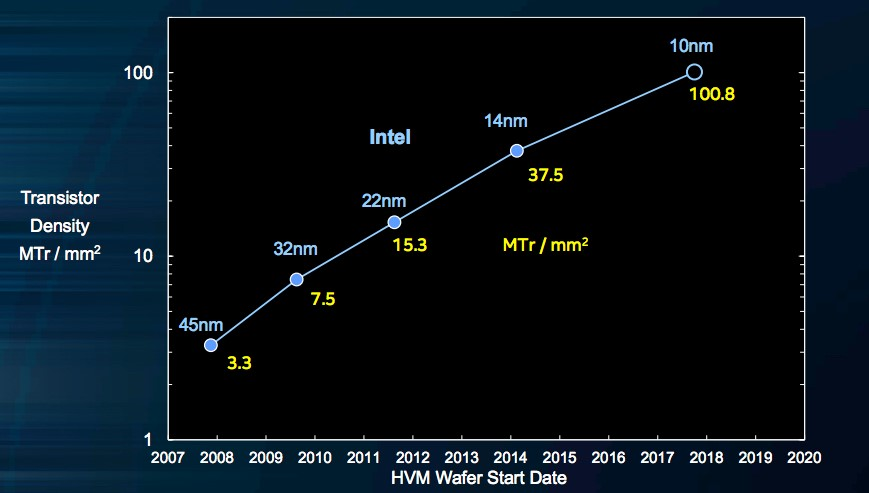
\includegraphics[width=\linewidth]{transistor.jpg}
	\caption{Fonte: IEEE, 2017}
	\label{fig:graph1}
\end{figure}

Tal fato realmente aconteceu de lá até hoje, com o intuito de colocar mais transistores em um chip, a principal linha de pesquisa para o desenvolvimento do poder computacional se baseava em como fazer transistores cada vez menores. Porém já é previsto há alguns anos que essa lei está pode se tornar invalida devido ao ponto que chegamos na redução de tamanho dos transistores. 

Com o tamanho dos transistores reduzindo exponencialmente, começou-se a perceber que em determinado ponto seria difícil ou até mesmo impossível conseguir bloquear a energia elétrica devido às propriedades da mecânica quântica, como o tunelamento quântico, onde um elétron tem a possibilidade de “pular” a barreira do transistor mesmo com ele “desligado”, e essa probabilidade é inversamente proporcional à espessura da barreira, ou seja, quanto mais fina, maior a probabilidade disso acontecer, passando informações incorretas. 

Entre esse e outros problemas gerados com a alta densidade de transistores, como por exemplo o superaquecimento, começou-se a pensar em novas formas de desenvolver o poder computacional, como transistores à base de outro material que não seja o silício, transistores com uma estrutura diferenciada, ou até mesmo a computação quântica, um tipo de computação que tem um princípio totalmente à parte da computação convencional.
Com o aumento de pesquisas na área da computação quântica, ela vem se tornando cada vez mais possível de ser uma das opções para o futuro, e atualmente vem mostrando um grande potencial quando utilizada para certos tipos de operações.
Na teoria, a computação quântica pode chegar a ser milhares de vezes mais rápida que a convencional, pelo fato de ter seu poder de processamento exponencialmente proporcional à quantidade de qubits utilizados, pois, diferentemente da convencional, ele trata não trata os bits apenas como 0 e 1, mas sim como a superposição dos bits através de sua probabilidade. 

O grande desafio para o desenvolvimento dessa nova tecnologia é como implementar essa teoria na pratica, e até que ponto os algoritmos da computação convencional podem ser remodelados para a quântica. Um dos métodos achados para representar o sistema de qubits foi através do spin de elétrons, mas ainda com muita dificuldade pois, atualmente, para conseguir resultados confiáveis, ou seja, sem interferência externa (ruído), é preciso isola-los e resfria-los à quase 0 Kelvin. Mas estima-se que um computador quântico funcional com 49 qubits já tem o poder de processamento equivalente aos computadores atuais. Em 2018, empresas como Google e IBM já anunciaram que desenvolveram chips quânticos na casa dos 70 e 50 qubits, porém ainda sem um total controle dos qubits, que, ao serem colocados em conjunto dificulta a tarefa de conseguir uma resposta limpa, sem “ruídos”. 

Junto a essa evolução, veio o aumento da preocupação em até que ponto ela seria uma ameaça para os algoritmos de encriptação atuais, que é o que possibilita a utilização da internet para troca de informações sigilosas, sejam elas transações bancarias, e-mails, documentos pessoais ou até mesmo documentos sigilosos de grandes empresas ou do governo.

\chapter{Objetivos}

\index{geral}O objetivo deste projeto de pesquisa é apresentar uma revisão sobre os aspectos fundamentais da computação quântica, tais como seu funcionamento e representação em comparação com o modelo de computação clássica adotado no século XXI, suas consequências em certos aspectos sociais contemporâneos, como segurança, privacidade de dados e informar sobre o avanço da computação pós-quântica frente a ameaça da quebra de algoritmos clássicos da criptografia. 

\chapter{Fundamentação Teórica}

Primordialmente, para a computação quântica ser entendida em sua essência, é necessário se entender o comportamento da realidade frente as regras da mecânica quântica. Diferentemente da mecânica clássica, uma mecânica determinista, onde é possível determinar o estado de uma partícula ao longo do tempo, ou até mesmo prever sua posição ou velocidade num futuro, a mecânica quântica se comporta de uma maneira antagônica ao determinismo, nela é impossível determinar o estado de uma partícula, apenas suas probabilidades, seja de posição ou de velocidade.

A evidencia de tais fatos começaram a surgir em 1927, com o enunciado da mecânica quântica, Princípio da incerteza, por Werner Heisenberg, um físico teórico alemão responsável pela criação da mecânica quântica. Tal princípio estabelece limites em que propriedades de uma partícula tais como posição e momento linear podem ser determinados. Em suma é evidenciado que dois estados de uma partícula não podem ser determinados ao mesmo tempo, quanto menor for a incerteza de um determinado estado, maior será a incerteza de seu par. Paralelamente, foi evidenciado que a medição perturba o estado quântico, ou seja os possíveis estados de uma partícula são destruídos após uma observação.

\section{O Gato de Schrödinger}

\begin{figure}[ht!]
	\centering 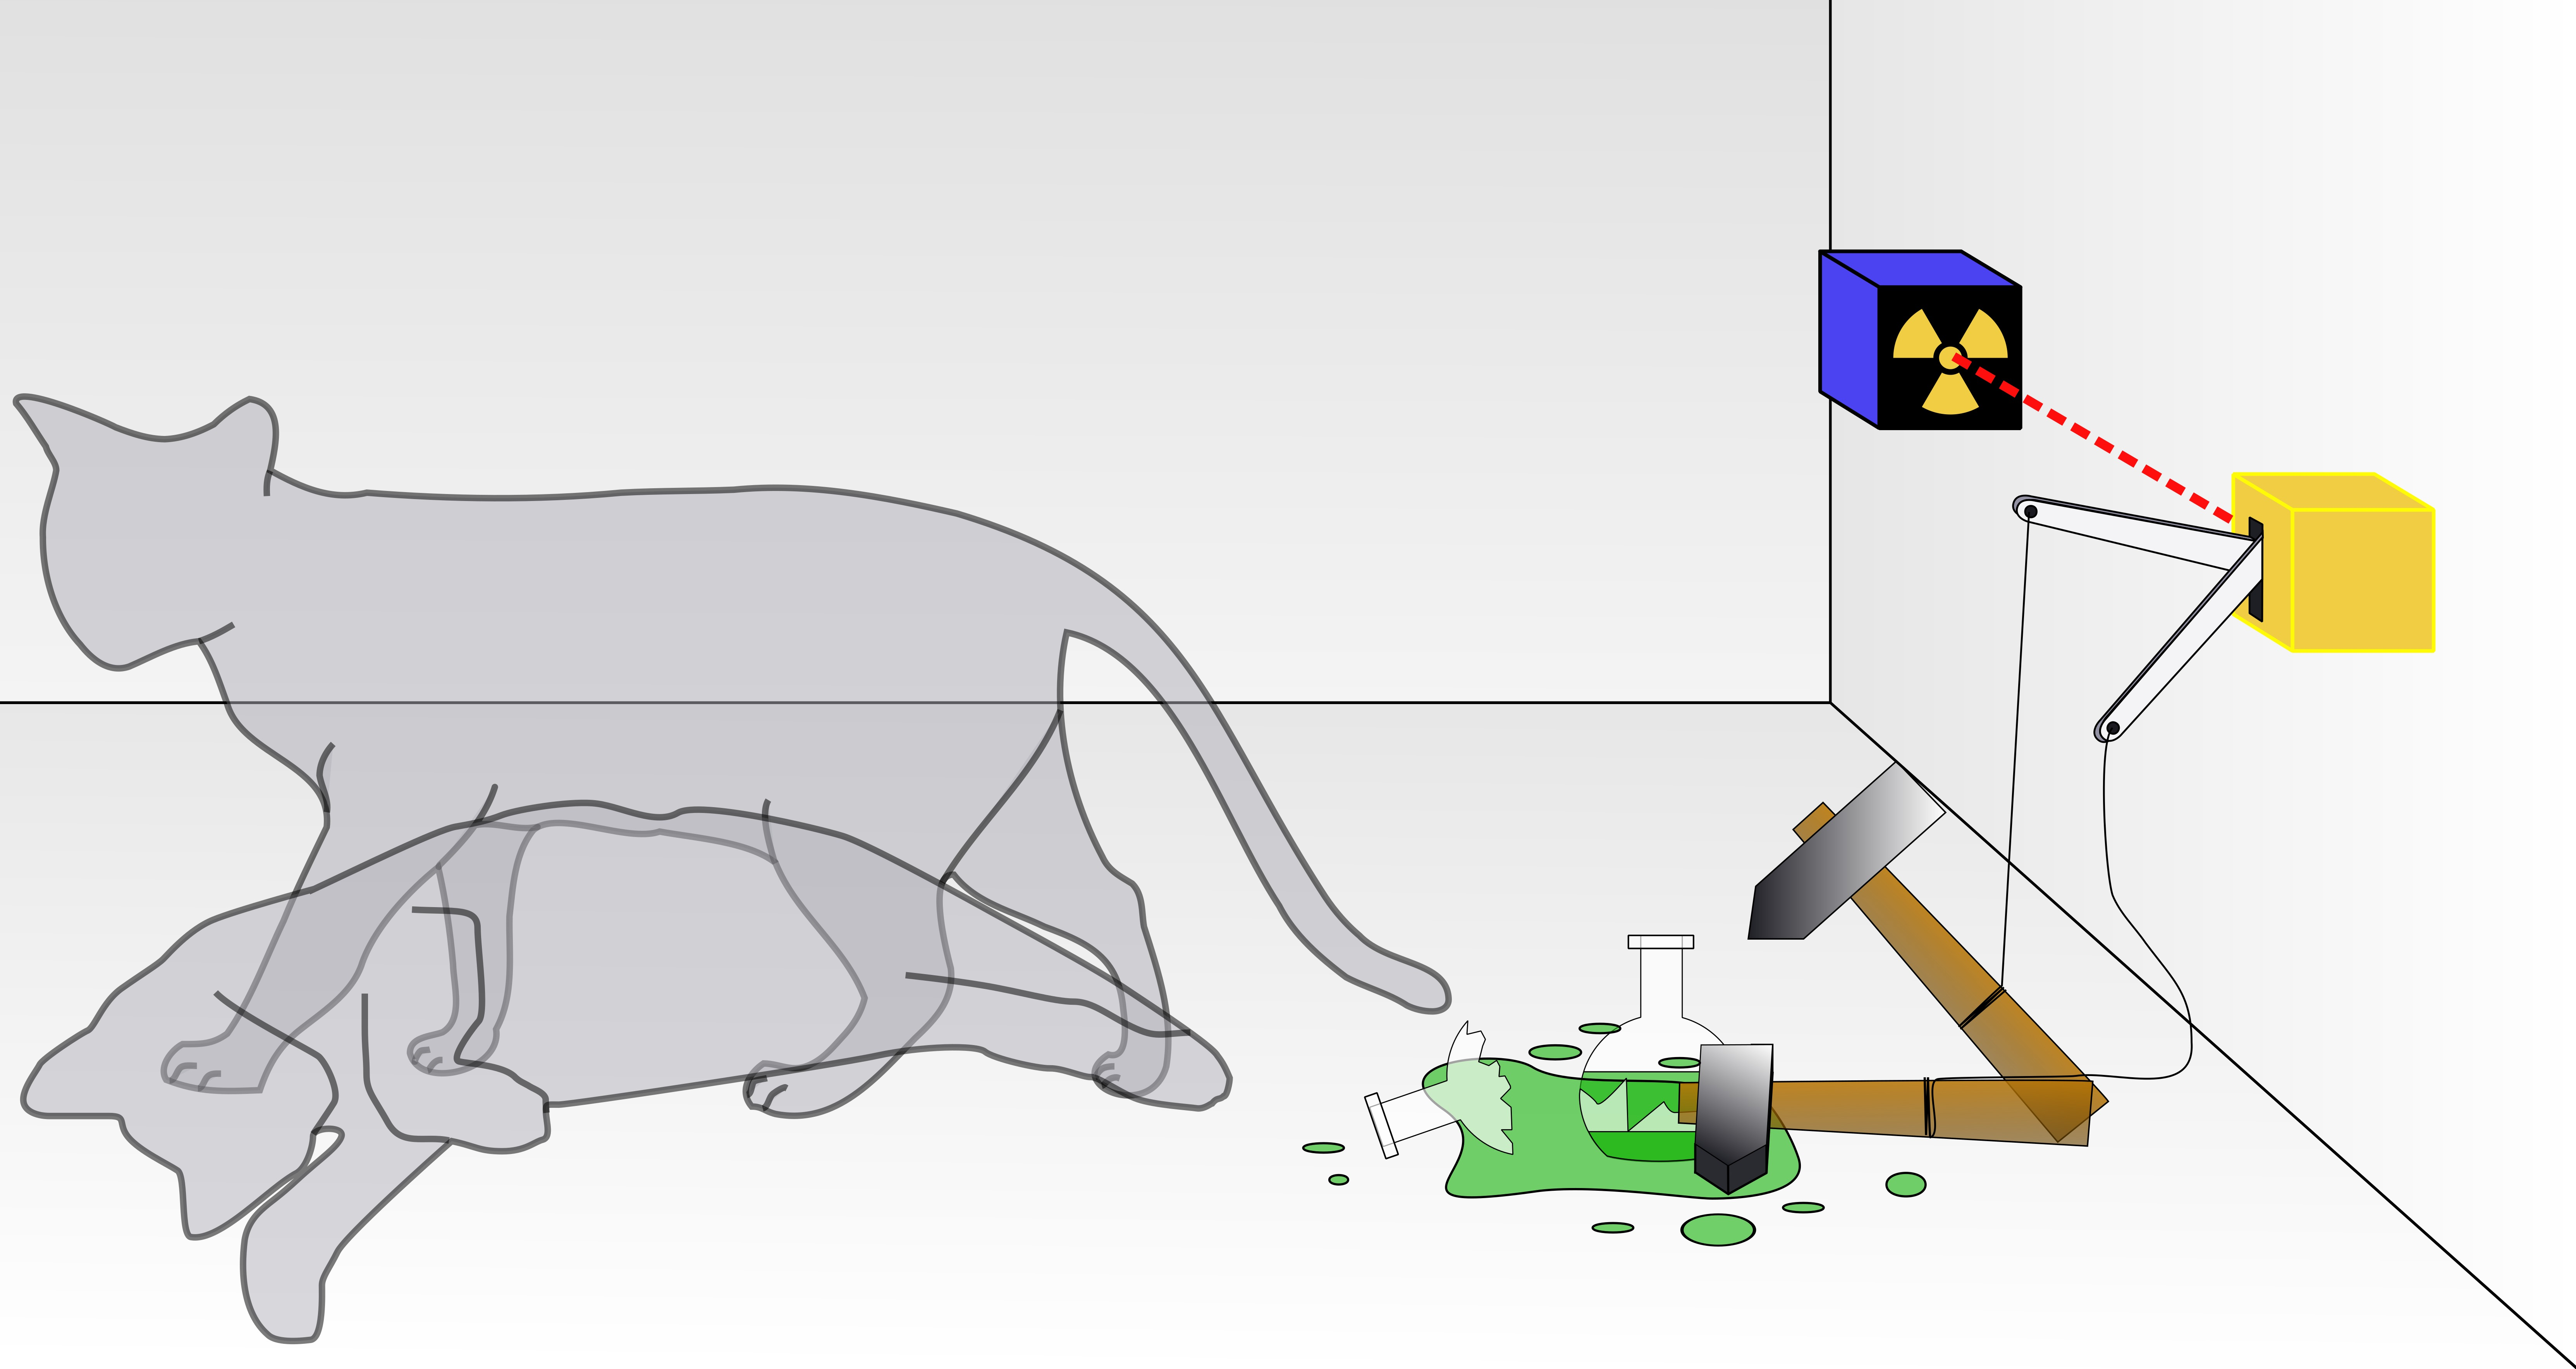
\includegraphics[width=\linewidth]{sobreposicao.jpg}
	\caption{Fonte: Wikipédia, 2008}
	\label{fig:gato}
\end{figure}

Embasado nessas ideias, Erwin Schrödinger, um físico teórico austríaco. Propôs um experimento lógico denominado, O Gato de Schrödinger: Suponha que exista um gato dentro de uma caixa – protegida contra interferência quântica – junto a um núcleo radioativo, um detector de radiação,  e um frasco de veneno letal ao gato. Logo, existem duas possiblidades, a primeira, caso o núcleo não decaia, não será detectada radiação, o frasco de veneno não será quebrado e o gato ficará vivo, ou a segunda, onde o núcleo decairá, será detectada radiação e o frasco irá quebrar, por conseguinte o gato morrerá. O ponto crítico dessa experiencia é baseado em tal questionamento: “Após algumas horas, o gato estará morto ou vivo?”. De acordo com Erwin Schrödinger, a nível quântico é possível o gato estar morto e vivo simultaneamente até abrirmos a caixa e essa observação destruiria o estado quântico de sobreposição do gato.

Essa simultaneidade se dá graças a coerência quântica, o estado onde a particula se mantém livre de perturbações do meio ambiente, como o vento ou o contato com a terra. Ao observar a particula (no caso abrir a caixa), o sistema irá ser perturbado, detruindo a coerência quântica.

\section{Tunelamento Quântico}
Analogamente a experiencia, partimos da visão de sobreposição de estados para o efeito de Tunelamento quântico, isto é, se partimos do meio da mecânica clássica, suponha que exista uma partícula que viaja no espaço com velocidade constante e exista uma barreira no meio desse espaço, logo, é evidente que se a partícula porta uma energia menor do que a energia da barreira, ela irá rebater na barreira e voltar. Porém, no âmbito quântico, se jogarmos um elétron contra uma barreira existe uma probabilidade finita e não nula, da partícula atravessar. 

\begin{figure}[h!]
	\centering
	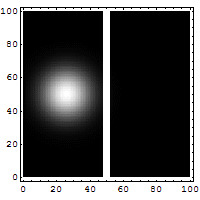
\includegraphics[scale=1]{tunelj1.jpg}
	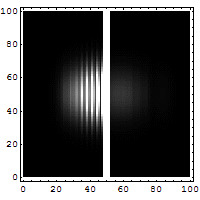
\includegraphics[scale=1]{tunelj2.jpg}
	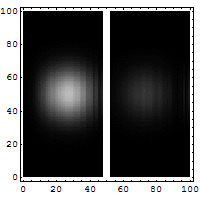
\includegraphics[scale=1]{tunelj3.jpg}		
	\caption{Fonte: Wikipédia, 2006}
	\label{fig:tunel0}
\end{figure}

Em síntese, o elétron atravessou e rebateu na barreira simultaneamente, o chamado Tunelamento quântico.

É completamente embasado nessas ideias que o computador quântico trabalha não mais com o bit clássico, mas sim com o qubit, que pode assumir todos os estados possíveis de uma palavra ao mesmo tempo, por exemplo, suponha uma palavra formada por dois qubits, pelas propriedades no supracitado, tal palavra pode assumir os quatro estados possíveis ao mesmo tempo: 00, 01, 10, 11. E consequentemente poderia ser encontrado qualquer um desses pares, em apenas uma passada. Matematicamente, segundo \cite{nielsen:2010} Nielsen (2010), esse fenômeno é chamado de superposição, que é a combinação linear dos estados dos qubits.

\chapter{Criptografia}

Sabendo que o poder computacional de um computador quântico é exponencialmente proporcional ao número de bits quânticos operacionais, diferentemente do computador normal onde é linearmente proporcional ao número de bits, é de se esperar que possamos ter problemas relacionados à quebra de segurança devido à enorme diferença entre os dois. Antes mesmo dessa nova tecnologia começar a se tornar realidade, já existiam pesquisadores pensando em como funcionaria os algoritmos onde houvesse a superposição dos bits, mesmo sem saber como de fato os qubits seriam fisicamente implementados. Um famoso exemplo é o algoritmo de Shor, proposto em seu artigo (1995), onde é mostrado como fazer a fatoração de um número utilizando qubits, o que é a base para quebrar um dos tipos de encriptação mais utilizado, o RSA. Mais especificamente, para quebrar esse algoritmo é preciso lidar com a fatoração de números primos enormes, o que poderia levar até centenas de milhares de anos para computadores convencionais atuais, mas já se sabe que utilizando computadores quânticos e o algoritmo de Shor, por exemplo, o problema que tem solução em tempo exponencial, passa a ser polinomial.

Para se ter uma ideia, a maior chave RSA decodificada que se têm notícia tinha 232 dígitos (768 bits), em novembro de 2009, utilizando centenas de processadores durante um período de 2 anos. Foi previsto que, com sorte, seria possível quebrar uma chave de 1024 bits na década seguinte dependendo da evolução dos algoritmos de fatoração e do poder computacional, mas ainda hoje isso não foi feito. O que garante que chaves RSA de 2048 bits ou maiores estão longe de serem consideradas frágeis para computadores convencionais.

Mesmo com o tempo de quebra das chaves RSA se tornando polinomial, os algoritmos de criptografia atuais que usam criptografia simétrica ou funções hash (não é o caso do RSA), com o tamanho das chaves dobradas, ainda são considerados seguros para os computadores quânticos iniciais. 

No entanto, devido à rápida evolução da computação quântica, a preocupação em relação a isso se elevou e surgiu uma nova área de estudo chamada de criptografia pós-quântica, onde ja se estabeleceu um protocolo para garantir a segurança do que estar por vir. Nele, é estudado a possibilidade de fazer a criptografia utilizando a mesma tecnologia (mecânica quântica) que está sendo desenvolvida nos computadores. A ideia é utilizar o mesmo principio da quebra de estado quântico, ou seja, do mesmo modo que um elemento perde as propriedades quânticas ao ser observado, isso aconteceria analogamente quando alguem tentasse decifrar um objeto encriptado, invalidando o mesmo.


\include{abntex2-modelo-include-comandos}

% ---
% Finaliza a parte no bookmark do PDF
% para que se inicie o bookmark na raiz
% e adiciona espaço de parte no Sumário
% ---
\phantompart

% ---
% Conclusão
% ---
\chapter*[Considerações finais]{Considerações finais}
\addcontentsline{toc}{chapter}{Considerações finais}

\lipsum[31-33]

% ----------------------------------------------------------
% ELEMENTOS PÓS-TEXTUAIS
% ----------------------------------------------------------
\postextual

% ----------------------------------------------------------
% Referências bibliográficas
% ----------------------------------------------------------

\bibliographystyle{apalike}
\bibliography{quantica}


\phantompart



\end{document}
